\chapter{Vierdimensionale ruimte}
\vspace{-1cm}\begin{flushright}
{\it `From henceforth, space by itself, and time by itself, \\ have vanished into the merest shadows \\ and only a kind of blend of the two exists in its own right'} \\ H. Minkowski
\end{flushright}
Een `gebeurtenis' vindt plaats op een bepaalde locatie, beschreven door
co\"ordinaten $(x,y,z)$, en op een bepaald tijdstip, beschreven door
co\"ordinaat~$t$. Voor de beschrijving van een gebeurtenis zijn dus in
totaal vier co\"ordinaten nodig. We zullen de co\"ordinaten van een
gebeurtenis noteren als $(ct,x,y,z)$, waarbij de tijd $t$ is
vermenigvuldigd met de lichtsnelheid $c$ (constant in elk
inertiaalsysteem) om de dimensie van elk van de vier co\"ordinaten
hetzelfde te laten zijn, namelijk die van een afstand.

Voorbeelden van gebeurtenissen zijn de flits van een lampje, of de
botsing tussen twee auto's. Om deze gebeurtenissen te tekenen in een
stelsel maken we gebruik van het $(ct,x)$ diagram, waarbij we de twee
resterende ruimtelijke co\"ordinaten $y$ en $z$ voor het gemak
weglaten. Een gebeurtenis is in het $(ct,x)$ diagram een punt. Een
continue, aaneengeschakelde stroom van gebeurtenissen van een voorwerp
vormt de wereldlijn van dit voorwerp. Dit is in het algemeen een
kromme lijn in het $(ct,x)$ vlak. In figuur~\ref{f:grid0} is het
$(ct,x)$ vlak getekend met een gebeurtenis en een aantal wereldlijnen.

\begin{figure}[ht] 
\centering
%\includegraphics[width=.7\textwidth]{syllabus.pictures/GridS0}
\epsfig{file=GridS0.pdf, width=0.7\textwidth}
\caption{{\sl \label{f:grid0} Het $(ct,x)$ vlak met een gebeurtenis
$A$, een stilstaand voorwerp $B$, een bewegend en versnellend voorwerp
$C$ en een lichtstraal $D$. In het rechterfiguur worden bij $E$ twee
deeltjes gecre\"eerd, bijvoorbeeld een positron en een elektron en
vliegen met tegengestelde snelheid weg. In $F$ botsen twee deeltjes,
waarbij hun snelheden omkeren.}}
\end{figure}

Het is duidelijk dat hoe kleiner de hoek van de wereldlijn met de
$x$-as is, hoe groter de snelheid is. Een horizontale lijn kan niet;
het zou een oneindige snelheid betekenen. De minimale hoek van een
wereldlijn met de $x$-as is 45$^o$, wanneer de snelheid $c$ is.


We kunnen dit soort diagrammen voor stelsel $S$ en $S'$ maken. De
transformatie tussen de co\"ordinaten van beide stelsels wordt
natuurlijk gegeven door de Lorentztransformaties. We nemen als
voorbeeld een waarnemer $A$ op aarde en een waarnemer $B$ in een raket
die met snelheid $\beta=2/3$ wegvliegt van $A$. Na drie jaar heeft de
raket dus een afstand van 2 lichtjaar afgelegd, in aardse co\"ordinaten
(stelsel $S$). De posities van $A$ en $B$, in stelsel $S$, zijn
weergegeven in het linker figuur~\ref{f:grid1}. De punten $A$ en $B$
zijn gelijktijdig in dit stelsel.


\begin{figure}[ht] 
\centering
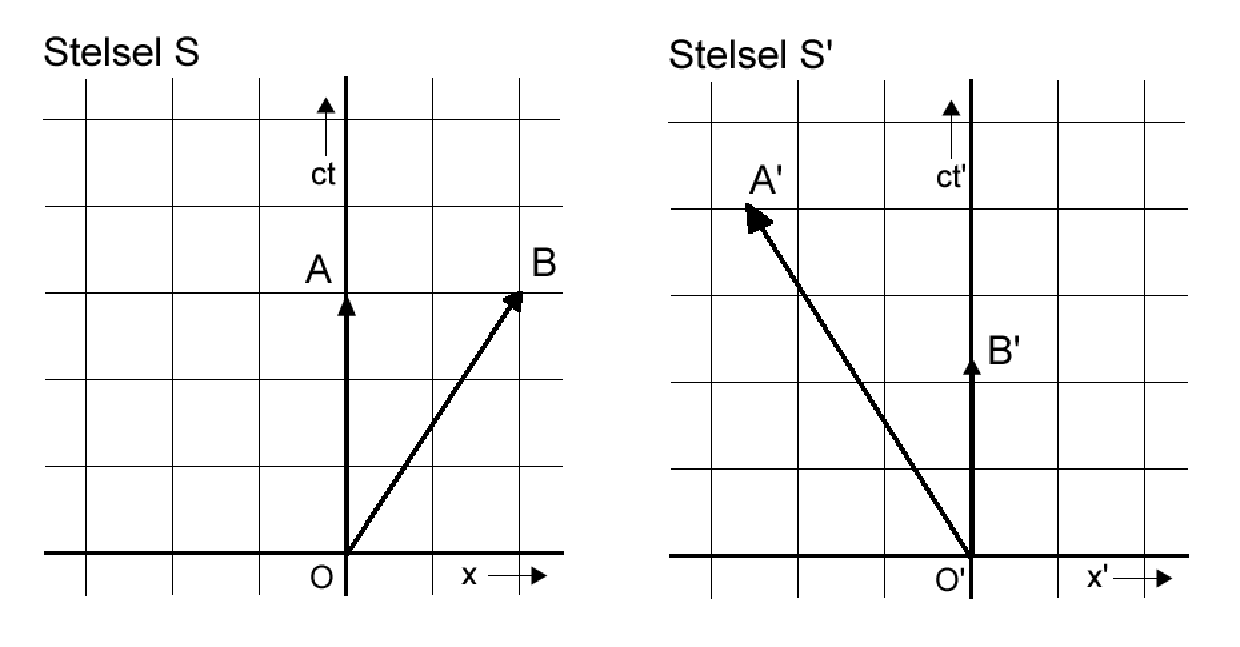
\epsfig{file=GridS1.pdf, width=0.8\textwidth}
\caption{{\sl \label{f:grid1} Wereldlijnen van waarnemer $A$ en $B$ uitgedrukt in stelsel $S$ en in stelsel $S'$.}}
\end{figure}

We kunnen nu de Lorentztransformaties gebruiken om de posities van $A$ en $B$ in het ruststelsel van de raket te bepalen (stelsel $S'$). De Lorentztransformaties geven:
\begin{eqnarray}\nonumber
A: \left(\begin{array}{c} ct \\ x \\ y \\ z \end{array}\right) &=&  
  \left(\begin{array}{c} 3 \\ 0 \\ 0 \\ 0 \end{array}\right) \mbox{lj} \\ \nonumber
A':  \left(\begin{array}{c} ct' \\ x' \\ y' \\ z' \end{array}\right) &=&  
  \left(\begin{array}{cccc} \gamma & -\beta \gamma & 0 & 0 \\ -\beta\gamma & \gamma & 0 & 0 \\ 0 & 0 & 1 & 0 \\ 0 & 0 & 0 & 1 \end{array}\right)
\left(\begin{array}{c} 3 \\ 0 \\ 0 \\ 0 \end{array}\right) =
\left(\begin{array}{c} 3\gamma \\ -2 \gamma \\ 0 \\ 0 \end{array}\right) \approx \left(\begin{array}{c} 4,02 \\ -2,68 \\ 0 \\ 0 \end{array}\right) 
 \mbox{lj}
\end{eqnarray}
en voor $B$ geeft dit (we laten nu de co\"ordinaten $y$ en $z$ weg)
\begin{eqnarray}\nonumber
B: \left(\begin{array}{c} ct \\ x \end{array}\right) &=&  
  \left(\begin{array}{c} 3 \\ 2 \end{array}\right) \mbox{lj} \\ \nonumber
B':  \left(\begin{array}{c} ct' \\ x' \end{array}\right) &=&  
  \left(\begin{array}{cc} \gamma & -\beta \gamma \\ -\beta\gamma & \gamma \end{array}\right)
\left(\begin{array}{c} 3 \\ 2 \end{array}\right) =
\gamma \left(\begin{array}{c} 5/3 \\ 0  \end{array}\right) \approx \left(\begin{array}{c} 2,23 \\ 0 \end{array}\right) 
 \mbox{lj}
\end{eqnarray}

De posities $A'$ en $B'$ zijn weergegeven in het
rechterfiguur~\ref{f:grid1}. Merk op dat in dit stelsel $A'$ en $B'$
niet meer gelijktijdig zijn.

\section{Causaliteit en de lichtsnelheid}
In het volgende verhaal willen we duidelijk maken dat de snelheid van
het licht de hoogste snelheid is waarmee informatie kan worden
overgedragen. We zullen dit laten zien aan hand van een tegenspraak:
als informatie sneller dan het licht zou kunnen worden overgedragen,
leidt dit tot verwarring van `oorzaak en gevolg'
(causaliteit). Causaliteit is een zeer fundamenteel principe in de
natuurkunde.  De `oorzaak' van een gebeurtenis vindt altijd plaats
voor het `gevolg'. Schending van causaliteit wordt nooit geaccepteerd
omdat dit leidt tot logische tegenspraak.  Het zou in principe immers
betekenen dat u uw voorouders kunt ombrengen voordat u geboren wordt.

Stel Anne en Frank zijn zijn vrienden. Frank gaat op ruimte reis met
een schip dat een snelheid van $\beta=0,6$ heeft (gebeurtenis $A$).  Na 4 jaar wachten
besluit Anne een brief aan Frank te sturen, met een nieuw type raket dat met
$\beta=3$ (!) kan reizen. Het moment van vertrek van deze raket noemen we $t=0$ en is gebeurtenis $B$.
Na 1 jaar in deze super-luminale raket is de brief bij Frank aangekomen (gebeurtenis $C$).

\begin{figure}[ht] 
\centering
%\includegraphics[width=.8\textwidth]{syllabus.pictures/GridS3}
\epsfig{file=GridS3.pdf, width=0.8\textwidth}
\caption{{\sl \label{f:grid3} Wereldlijnen van Anne ($A-B$), van Frank
($A-C$) en van de brief ($B-C$). Aan de linkerkant in het
co\"ordinatenstelsel in rust t.o.v. Anne, rechts in rust t.o.v. Frank. Frank
ziet de brief `uit de toekomst' komen.}}
\end{figure}


In het co\"ordinatenstelsel van Anne heeft Frank dus in 5 jaar een
totale afstand van 3 lj afgelegd, en ontvangt Frank de brief een jaar
nadat hij is verstuurd. Deze situatie is in weergegeven in het
linkerfiguur~\ref{f:grid3}. Maar in het stelsel in rust ten opzichte
van Frank, $S'$, is de situatie anders. Via de Lorentztransformaties
volgt:
\begin{eqnarray}\nonumber
A: \left( \begin{array}{c} ct \\ x \end{array} \right) = 
  \left( \begin{array}{c} -4 \\ 0 \end{array} \right) & \rightarrow & A': 
\left( \begin{array}{cc} \gamma & -\beta\gamma \\ -\beta\gamma & \gamma \end{array} \right)  
\left( \begin{array}{c} -4 \\ 0 \end{array} \right) = 
\left( \begin{array}{c} -5 \\ 3 \end{array} \right)  \\\nonumber
\end{eqnarray}
en evenzo voor $B'=(0,0)$ en $C'=(-1,3)$. In het co\"ordinatenstelsel
$S'$ bereikt Frank punt $C'$ eerder dan de brief die is verstuurd. Met
andere woorden, in zijn inertiaalsysteem komt de brief eerder aan dan
hij is verstuurd. Dit is in tegenspraak met causaliteit en daarmee
onmogelijk. Het is het gevolg van de aanname dat de brief met
$\beta=3$ werd verstuurd, en er kan geconcludeerd worden dat geen
informatie kan worden overgebracht met een snelheid groter dan $c$.

Merk op dat er overigens fenomenen in de natuur te vinden zijn die
wel sneller gaan dan de snelheid van het licht. Denk bijvoorbeeld aan
een lichtvlek die de lichtbundel van een vuurtoren maakt op een ver
weg gelegen eiland. Omdat de lichtbundel ronddraait zal de snelheid
waarmee de lichtvlek zich beweegt groter worden naarmate de afstand
tot de vuurtoren toeneemt. Er is geen limiet voor de snelheid van de
lichtvlek. Maar er wordt hierbij geen informatie overgedragen die
sneller gaat dan $c$!


\section{Minkowski-diagrammen}
In plaats van het tekenen van twee diagrammen voor de stelsels $S$ en
$S'$, kunnen beide stelsels ook in \'e\'en diagram getekend
worden. Dit wordt het Minkowski diagram genoemd.  Met deze ruimte-tijd
diagrammen kunnen de meeste vraagstukken van de speciale
relativiteitstheorie worden weergegeven, en deze geometrische
benadering is de meest elegante manier om de vraagstukken op te
lossen. Het is robuust omdat het inlevingsvermogen vraagt om de relatie
tussen gebeurtenissen en wereldlijnen te visualiseren.

 
Indien we het $(x,\ ct)$ vlak voorstellen m.b.v. twee loodrecht op
elkaar staande assen zoals in fig.~\ref{f:conseq2} dan wordt in deze
figuur de $x^{'}$-as beschreven door een lijn die volgt uit de eis
$ct^{'} = 0$, dus (zie formule \ref{v:lorentz11}.) $ct = \beta x$,
m.a.w. door een lijn met richtingsco\"{e}ffici\"{e}nt $\beta$.  Op
analoge wijze vinden we de lijn die de $ct^{'}$ as beschrijft uit de
eis $x^{'} = 0$, dus (zie formule \ref{v:lorentz10}.)  $x = \beta ct$,
of $ct = \frac{x}{\beta}$.  Dit is een lijn met
richtingsco\"{e}ffici\"{e}nt $\frac{1}{\beta}$.  D.w.z. de $x^{'}$-as
maakt met de $x$-as een hoek $\alpha$ z\'{o}, dat  $\tan \alpha = \beta$
en de $ct^{'}$-as maakt met de $ct$-as dezelfde hoek $\alpha$ zoals in
figuur \ref{f:conseq2} (Ga na.)\footnote{Op de website \url{www.nikhef.nl/\string~stanb/Minkowski.html} vindt u een flash animatie van het Minkowski-diagram.}.

% \begin{figure} [h]
% \begin{center}
% \mbox{\epsfxsize=8cm\epsffile{syllabus.pictures//minkowski.eps}}
% \caption{Minkowski diagram}
% \label{f:conseq2}
% \end{center}
% \end{figure}

\begin{figure}[ht]
\centering
%\includegraphics[width=.49\textwidth]{syllabus.pictures/minkowski}
\epsfig{file=minkowski.pdf, width=0.49\textwidth}
\caption{{\sl Minkowski-diagram}}
\label{f:conseq2}
\end{figure}


In figuur \ref{f:conseq2} is ook aangegeven de lijn $x = ct$:
de relatie tussen plaats en tijd voor een lichtstraal.
Deze lijn wordt ook wel als de lichtkegel aangeduid.
Twee `gebeurtenissen' $A$ en $B$ worden verbonden door een zogenaamde 
wereldlijn.
De lijn $AB$ in figuur \ref{f:conseq2} zou een eenparig bewegend deeltje kunnen voorstellen.
Verder is in de figuur aangegeven hoe het punt $(ct,x) = (1, 0)$ 
transformeert naar 
$(ct',x^{'}) = (\gamma,-\beta \gamma )$. 
(Ga na m.b.v. de Lorentztransformatie.)

%aanvulling september 2001
Het is gemakkelijk in te zien dat de eenheid van tijd (uitgedrukt in
$ct$) weergegeven t.o.v. systeem $S$ voor alle andere systemen $S'$
die t.o.v. $S$ eenparig langs de $x$-as bewegen op een hyperbool
liggen.  Immers: de grootheid $s^2=(ct)^2-x^2-y^2-z^2$ is een
invariant en deze vergelijking beschrijft een hyperbool in het
$(x,\ ct)$ vlak. We kunnen bijvoorbeeld nemen $(ct)^2-x^2=1$ en
verkrijgen zo de twee parabolen aangegeven in figuur~\ref{f:mink} (links) met
een `+'. Alle punten op deze parabool hebben dus dezelfde waarde voor
$s^2$. Een Lorentztransformatie van stelsel $S$ naar $S'$ is een
verschuiving langs deze parabolische baan.

Voor negatieve $s^2$ hebben we als karakteristieke hyperbool de
vergelijking $(ct)^{2}-x^2 = -1$, aangegeven in het figuur met een `-'
teken.

De lijnen voor $s^2=0$ zijn de wereldlijnen van die van het licht, en
komen overeen met de diagonale lijn van het figuur. Zij vormen de
`lichtkegel'. De lichtkegel is duidelijker als kegel te visualiseren
in de $(ct,x,y)$ ruimte, d.w.z., wanneer er twee ruimtelijke dimensies
getekend worden, zoals in figuur~\ref{f:mink} (rechts).

% \begin{figure} [h]
% \begin{center}
% \mbox{\epsfxsize=8cm\epsffile{syllabus.pictures//minkowski2.eps}}
% \caption{Hyperbolen in systeem $S$ waarop de co\"{o}rdinaten $ct' = 1$ 
% (hyperbolen aangegeven met '-') resp. $x' = 1$ (hyperbolen aangegeven
% met een '+') van alle mogelijke systemen $S'$ liggen.}
% \label{f:mink}
% \end{center}
% \end{figure}

\begin{figure}[ht]
\centering
%\includegraphics[width=.49\textwidth]{syllabus.pictures/minkowski2}
\epsfig{file=minkowski2.pdf, width=0.49\textwidth}
%\includegraphics[width=.49\textwidth]{syllabus.pictures/GridS5}
\epsfig{file=GridS5.pdf, width=0.49\textwidth}
\caption{{\sl Links: hyperbolen in systeem $S$ waarop de co\"{o}rdinaten $ct' = 1$ 
(hyperbolen aangegeven met '-') resp. $x' = 1$ (hyperbolen aangegeven
met een '+') van alle mogelijke systemen $S'$ liggen. Rechts: de lichtkegel voor co\"ordinaten $(ct,x,y)$.}}
\label{f:mink}
\end{figure}


Voor punten die `in' de lichtkegel liggen, dus in het gebied tussen de
asymptoten van de met `+' gelabelde hyperbolen, geldt dat er altijd
een Lorentztransformatie gevonden kan worden z\'{o} dat het punt in
het systeem $S'$ op de $ct'$-as ligt.  Viervectoren overeenkomend met
dergelijke punten noemen we tijdachtig (`timelike'). Gebeurtenissen in
elkaars lichtkegel volgen elkaar op, en er kan geen verwarring
ontstaan over welke gebeurtenis eerder of later plaatsvond. Wel kan het
onderlinge tijdsverschil veranderen indien het bekeken wordt vanuit een ander
stelsel, maar er is geen transformatie die de {\it volgorde} in de
tijd van de punten veranderd.  De gebeurtenissen zijn `causaal
verbonden', d.w.z. de gebeurtenis die eerder plaatsvond kan (mogelijkerwijs) invloed
hebben op een gebeurtenis die later plaatsvond: de informatie-overdracht van de eerste naar 
de tweede gebeurtenis kan slechts langzamer dan $c$ verlopen.



Viervectoren met co\"{o}rdinaten `buiten' de lichtkegel noemen we,
uiteraard, ruimteachtig (`spacelike'). Twee gebeurtenissen die een
onderlinge `ruimteachtige' afstand tot elkaar hebben kunnen elkaar op geen enkele manier
beïnvloeden en zijn hiermee dus niet causaal verbonden. De volgorde in
de tijd tussen deze gebeurtenissen hangt af van het stelsel waarin ze
beschreven worden. 


%einde aanvulling september 2001

Minkowski-diagrammen illustreren op heldere wijze allerlei
 kwalitatieve eigenschappen van de Lorentztransformatie, zoals de 
betrekkelijkheid van het begrip gelijktijdigheid (ga na) e.d.
In zekere zin zijn deze diagrammen echter ook verraderlijk, omdat de meetkunde 
van ruimte-tijd niet dezelfde is als de meetkunde van de ruimte alleen.
In het bijzonder is de grootte van een plaatsvector 
$\vec{r} = (x, y, z)$ gelijk aan $|\vec{r}| = \sqrt{x^{2} + y^{2} + z^{2}}$.
De grootte van de ruimte-tijd vector $r = (x, y, z, ct)$ is echter
$|r| = \sqrt{c^2 t^2 - x^{2} - y^{2} - z^{2}}$.
Deze grootte wordt dus berekend volgens een andere {\sl metriek}.
Om dit te ondervangen zette Minkowski zelf niet $ct$ maar $ict$ op de tijd-as
uit ($(ict)^{2} =  -c^{2}t^{2}$).
Dan is de standaard metriek te gebruiken. Deze truc is echter niet altijd vol
te houden.
We zullen de discussie hier niet verder voeren.

\subsection{Relativiteit van gelijktijdigheid}
We hadden eerder gezien dat gelijktijdigheid een relatief begrip is,
d.w.z., het hangt van het referentiestelsel van de waarnemer af of
twee gebeurtenissen gelijktijdig zijn of niet. We laten dat hier nogmaals
expliciet zien met gebruik making van ruimte-tijd diagrammen.

Hoe synchroniseren we twee klokken die op een afstand $l$ van elkaar
staan? Het meest eenvoudige is om een lamp in het midden te plaatsen,
het een lichtflits te laten uitzenden, en op het moment dat de
lichtflits aankomt beginnen de klokken te tikken. Het ruimte-tijd
diagram van deze situatie in het ruststelsel $S$ is getekend in
figuur~\ref{f:sync}, met de lamp in het midden en de twee klokken op
positie $\pm l/2$. De flits is gemarkeerd met F en het ontvangen van
de flits als G en H. Hierna beginnen de klokken te tikken zoals
aangegeven met stippen op de wereldlijn op de klok. Gelijktijdige
tikken liggen op de horizontale lijn die de tikken verbind, omdat zij
dezelfde tijd co\"ordinaat $ct$ hebben.

\begin{figure}[ht] 
\centering
%\includegraphics[width=.8\textwidth]{syllabus.pictures/Gelijktijdigheid}
\epsfig{file=Gelijktijdigheid.pdf, width=0.8\textwidth}
\caption{{\sl Het synchroniseren van twee klokken in stelsel $S$ dmv
het uitzenden van een lichtsignaal in het midden (F).  Elke klok
begint te tikken zodra de lichtflits is ontvangen (G en H). Lijnen van
gelijktijdigheid verbinden overeenkomstige tikken en zijn
horizontaal. \label{f:sync}}}
\end{figure}

Stel nu een ander referentiestelsel $S'$ voor, dat beweegt met een
snelheid $v=\beta c$ in de $x$-richting t.o.v. $S$.  In dit nieuwe
stelsel lopen de wereldlijnen van de klokken niet meer verticaal,
immers, zij verplaatsen met een snelheid $v$ als de tijd tikt. Volgens
het relativiteitsprincipe zullen de lichtsignalen nog steeds op lijnen
van 45$^o$ lopen. Het ruimte-tijd diagram in $S'$ ziet er dus uit
zoals in figuur~\ref{f:sync2}. Merk op dat de lijnen van
gelijktijdigheid scheef lopen in $S'$. Dit betekent dat twee
gebeurtenissen die simultaan zijn in $S$, in het algemeen niet meer
simultaan zijn in $S'$.

\begin{figure}[htb] 
\centering
%\includegraphics[width=.6\textwidth]{syllabus.pictures/Gelijktijdigheid2}
\epsfig{file=Gelijktijdigheid2.pdf, width=0.6\textwidth}
\caption{{\sl De klokken zoals geobserveerd in $S'$, samen met
gebeurtenissen F, G, H. Hoewel de klokken zijn gesynchroniseerd in
$S$, zijn ze dat niet in $S'$. Merk op dat de lijnen van
gelijktijdigheid scheef lopen in $S'$.\label{f:sync2} }}
\end{figure}

\subsection{De `ladder in de schuur'-paradox}
De boeren Niels (N) en Petra (P) hebben een schuur op het erf van
lengte $l$ en een ladder met lengte $2l$. Zij willen de ladder in de
schuur opbergen, maar deze is natuurlijk te lang. N stelt voor dat P
aankomt met de ladder met een snelheid $u=0,866c$. Bij deze snelheid
is $\gamma=2$ , en de ladder is met de Lorentzcontractie precies
genoeg korter geworden om in de schuur te passen. P heeft bezwaar. P
beargumenteerd dat als hij met de ladder aan het rennen is, in {\sl
zijn} co\"ordinatensysteem, de ladder nog steeds een lengte $2l$ heeft,
terwijl de schuur een Lorentzcontractie ondergaat en een lengte heeft
van $l/2$. Het plan om te gaan rennen met hoge snelheid heeft het
probleem alleen erger gemaakt.


Kunnen zij beide gelijk hebben? Stel voor dat P met de ladder
door de deur aan de voorkant van de schuur rent, en er via een andere
deur aan de achterkant weer uit komt. Stel verder voor dat de schuur
een mechaniek heeft waardoor de voordeur onmiddellijk sluit zodra de
achterkant van de ladder binnen is (noem dit gebeurtenis C), en een mechaniek waarmee de
achterdeur opent, precies op het moment wanneer de voorkant van de
ladder daar aangekomen is (gebeurtenis D). Er zijn nu twee
mogelijkheden: er is een tijd-interval waarin beide deuren gesloten
zijn of dit tijdsinterval is er
niet. Als dit tijdsinterval bestaat concluderen we dat de ladder past,
als het niet bestaat past de ladder niet. Wie heeft er gelijk?

\begin{figure}[ht] 
\centering
%\includegraphics[width=.8\textwidth]{syllabus.pictures/Schuurparadox}
\epsfig{file=Schuurparadox.pdf, width=0.8\textwidth}
\caption{{\sl Wereldlijnen van de voor- en achterkant van de schuur (G en H), en de voor en achterkant van de ladder (J en K) en gebeurtenissen 
C en D in het ruststelsel van N (figuur a) en in het ruststelsel van P (figuur b). Terwijl C en D gelijktijdig zijn in het stelsel van N,
zijn ze dit niet in het stelsel van P.\label{f:schuur}}}
\end{figure}


We kunnen ruimte-tijd plaatjes maken van de ladder en de schuur in
beide co\"ordinatenstelsels in rust voor N en P. In
figuur~\ref{f:schuur}, hebben de voor en achterkant van de schuur het
label G en H, en de voor en achterkant van de ladder label J en K. In
het co\"ordinatensysteem van N zijn inderdaad de gebeurtenissen C en D
gelijktijdig, dus is er een moment in de tijd van N dat de ladder in
de schuur past. In het stelsel van P echter, zijn deze gebeurtenissen
niet meer gelijktijdig! Gebeurtenis D vindt plaats v\`o\`ordat event C
plaatsvindt, dus is er geen tijd in het stelsel van P waarin de ladder
in zijn geheel in de schuur zit. Hiermee hebben beide waarnemers gelijk: de
vraag of de ladder in de schuur past is afhankelijk van het co\"ordinaten-stelsel;
het hangt af of twee gebeurtenissen gelijktijdig
zijn, en we hebben gezien dat gelijktijdigheid een relatief begrip is.
